\documentclass[oneside]{book}
\title{{\huge\bfseries Merlin's Compendium}}
\author{{\Large\itshape Ian Kuffel}}
\date{}

\usepackage{amsfonts,amssymb,amsthm,mathtools}
\usepackage{physics,braket,bm}
\usepackage[margin=0.75in]{geometry}
\usepackage{enumitem}
\usepackage{graphicx,float}
\usepackage{tabularx,makecell,array}
\usepackage[depth=3]{bookmark}

\newcolumntype{Y}{>{\centering\arraybackslash}X}

\numberwithin{figure}{section}
\numberwithin{equation}{section}

\renewcommand*{\thefootnote}{[\arabic{footnote}]}

\newcommand{\sq}{\subseteq}
\newcommand{\paren}[1]{\left(#1\right)}
\newcommand{\bhat}[1]{\bm{\hat{#1}}}
\newcommand{\eps}{\epsilon}
\newcommand{\veps}{\varepsilon}
\newcommand{\dpdv}{\displaystyle\pdv}
\newcommand{\skipline}{\newline\newline}

\theoremstyle{definition}
\newtheorem{definition}{Definition}[section]

\begin{document}
	\maketitle
	\bookmark[page=1]{Title Page}
	\tableofcontents
	\bookmark[page=2]{Table of Contents}
	\chapter*{Preface}
	\addcontentsline{toc}{chapter}{Preface}
	This is a compendium of all the physics and relevant mathematics that I have learned in the course of my undergraduate degree at Texas A\&M University. The goal is make a clear and concise explanation of various topics I learned during my undergraduate degree. This compendium can be used to refresh one's memory on the various topics and hopefully this will also serve as a useful guide to those just beginning to learn the topics that are covered in this compendium.

	\chapter{Coordinate Systems}

	\section{Cartesian Coordinates}
	The Cartesian coordinate system uses the standard $ x $, $ y $, and $ z $ directions. In physics, a common notation for the basis vectors are $ \bhat{i} \equiv \bhat{x} $, $ \bhat{j} \equiv \bhat{y} $, and $ \bhat{k} \equiv \bhat{z} $ to avoid confusion with the coordinate variables.
	\begin{figure}[H]
		\centering
		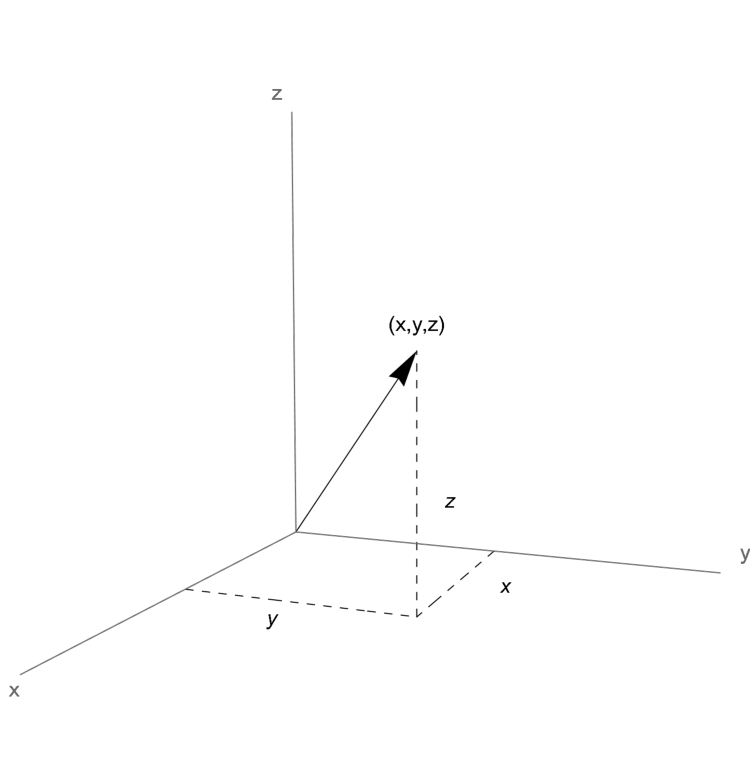
\includegraphics[width=0.6\columnwidth]{Figures/Coordinates/Cartesian Coordinates.pdf}
		\caption{Cartesian Coordinates.}
		\label{fig:cart}
	\end{figure}
	In Cartesian coordinates, we denote the vector with $ \bm{v} = x\bhat{i} + y\bhat{j} + z\bhat{k} = (x,y,z) $. The biggest advantage with this coordinate system is that the unit vectors do not change with respect to time. Thus, we can always change other coordinate systems back into Cartesian to see how they evolve with time.

	The cross products between the Cartesian coordinate vectors are:
	\begin{equation}\label{eq:cart_cross}
		\begin{cases}
			\bhat{x} \cross \bhat{y} &= \bhat{z}\\
			\bhat{y} \cross \bhat{z} &= \bhat{x}\\
			\bhat{z} \cross \bhat{x} &= \bhat{y}
		\end{cases}
	\end{equation}
	Using the relationship, $ \bm{A} \cross \bm{B} = \bm{C} \Leftrightarrow \bm{B} \cross \bm{A} = -\bm{C} $, you can derive the rest of the relationships from Eq. \ref{eq:cart_cross}. It is sometimes easier to write vectors and their relationships using Kronecher-Delta and Levi-Civita \footnote{See Appendix. \ref{sec:lckd}.}. Here are a list useful vector relationships:
	\begin{align}
		\bm{r} &= x\bhat{i} + y\bhat{j} + z\bhat{k}\\
		\dd{\bm{\ell}} &= \dd{x}\bhat{i} + \dd{y}\bhat{j} + \dd{z}\bhat{k}\\
		\dd{\tau} &= \dd{x}\dd{y}\dd{z}\\
		\grad{f} &= \pdv{f}{x}\bhat{i} + \pdv{f}{y}\bhat{j} + \pdv{f}{z}\bhat{k}\\
		\div{\bm{v}} &= \pdv{v_x}{x} + \pdv{v_y}{y} + \pdv{v_z}{z}\\
		\curl{\bm{v}} &= \paren{\pdv{v_z}{y} - \pdv{v_y}{z}}\bhat{i} + \paren{\pdv{v_x}{z} - \pdv{v_z}{x}}\bhat{j} + \paren{\pdv{v_y}{x} - \pdv{v_x}{y}}\bhat{k}
	\end{align}

	\section{Cylindrical Coordinates}
	Cylindrical coordinates are given by $ (\rho,\phi,z) $. This tends to be useful when you have a cylindrical object or some kind of cylindrical symmetry you want to describe. $ \rho $ corresponds to the radial length in the $ x-y $ plane, $ \phi $ is the angle with respect to the $ x $ axis, and $ z $ is of course the $ z $ coordinate from our Cartesian coordinates. For these coordinates, we will use the following unit vectors: $ \bhat{\rho} $, $ \bhat{\phi} $, and $ \bhat{z} $. These unit vectors are illustrated in the following figure:
	\begin{figure}[H]
		\centering
		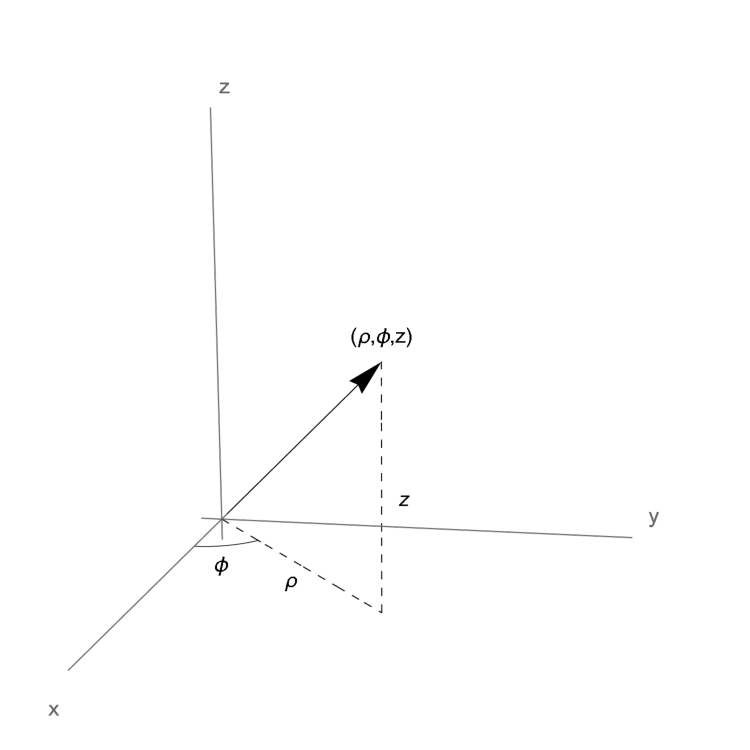
\includegraphics[width=0.6\columnwidth]{Figures/Coordinates/Cylindrical Coordinates.pdf}
		\caption{Cylindrical Coordinates.}
		\label{fig:cylind}
	\end{figure}

	The unit vectors are given by
	\begin{equation}
		\begin{cases}
			\bhat{\rho} &= \cos\phi\bhat{i} + \sin\phi\bhat{j}\\
			\bhat{\phi} &= -\sin\phi\bhat{i} + \cos\phi\bhat{j}\\
			\bhat{z} &= \bhat{k}
		\end{cases}
	\end{equation}
	Thus, conversions from cylindrical coordinates $ (\rho, \phi, z) $ to Cartesian coordinates $ (x,y,z) $ are given by:
	\begin{equation}
		\begin{cases}
			x &= \rho\cos\phi\\
			y &= \rho\sin\phi\\
			z &= z
		\end{cases}
	\end{equation}
	Conversions between the Cartesian unit vectors to cylindrical unit vectors are given by:
	\begin{equation}
		\begin{cases}
			\bhat{i} &= \cos\phi\bhat{\rho} - \sin\phi\bhat{\phi}\\
			\bhat{j} &= \sin\phi\bhat{\rho} + \cos\phi\bhat{\phi}\\
			\bhat{k} &= \bhat{z}
		\end{cases}
	\end{equation}
	Their cross product relationships are:
	\begin{equation}
		\begin{cases}
			\bhat{\rho} \cross \bhat{\phi} &= \bhat{z}\\
			\bhat{\phi} \cross \bhat{z} &= \bhat{\rho}\\
			\bhat{z} \cross \bhat{\rho} &= \bhat{\phi}
		\end{cases}
	\end{equation}
	Some useful vector relationships are:
	\begin{align}
		\bm{r} &= \rho\bhat{\rho} + z\bhat{z}\\
		\dd{\bm{\ell}} &= \dd{\rho}\bhat{\rho} + \rho\dd{\phi}\bhat{\phi} + \dd{z}\bhat{z}\\
		\dd{\tau} &= \rho\dd{\rho}\dd{\phi}\dd{z}\\
		\grad{f} &= \pdv{f}{\rho}\bhat{\rho} + \dfrac{1}{\rho}\pdv{f}{\phi}\bhat{\phi} + \pdv{f}{z}\bhat{z}\\
		\div{\bm{v}} &= \dfrac{1}{\rho}\pdv{\rho}\paren{\rho v_\rho} + \dfrac{1}{\rho}\pdv{v_\phi}{\phi} + \pdv{v_z}{z}\\
		\curl{\bm{v}} &= \left[\dfrac{1}{\rho}\pdv{v_z}{\phi} - \pdv{v_\phi}{z}\right]\bhat{\rho} + \left[\pdv{v_\rho}{z} - \pdv{v_z}{\rho}\right]\bhat{\phi} + \dfrac{1}{\rho}\left[\pdv{\rho}\paren{\rho v_\phi} - \pdv{v_\rho}{\phi}\right]\bhat{z}
	\end{align}

	\section{Spherical Coordinates}
	Similarly, spherical coordinates are useful to describing spherical objects or for things that have some sort of spherical symmetry (i.e., a force that depends only on the distance between the objects).
	
	For spherical coordinates, we use $ (r, \theta, \phi) $, where $ r $ is radius from the origin, $ \theta $ is the polar angle, and $ \phi $ is the azimuthal angle\footnote{Note that in most mathematical literature, the roles of $ \theta $ and $ \phi $ are reversed. As long as you know which is the azimuthal and which is the polar, you should be fine.}. Their respective unit vectors being: $ \bhat{r} $, $ \bhat{\theta} $, and $ \bhat{\phi} $.
	\begin{figure}[H]
		\centering
		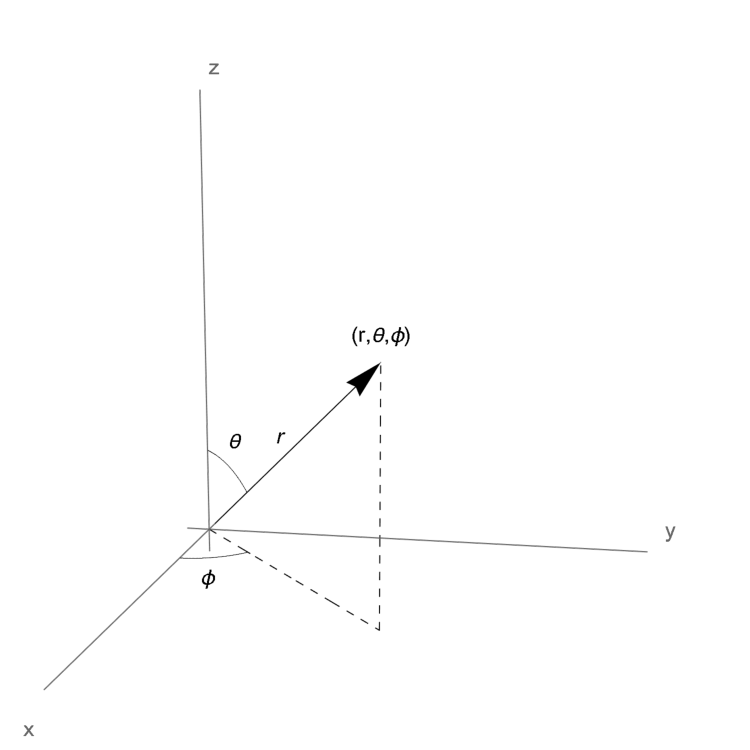
\includegraphics[width=0.6\columnwidth]{Figures/Coordinates/Polar Coordinates.pdf}
		\caption{Polar Coordinates.}
		\label{fig:polar}
	\end{figure}
	The unit vectors are given by
	\begin{equation}
		\begin{cases}
			\bhat{r} &= \cos\phi\sin\theta\bhat{i} + \sin\phi\sin\theta\bhat{j} + \cos\theta\bhat{k}\\
			\bhat{\theta} &= \cos\phi\cos\theta\bhat{i} + \sin\phi\cos\theta\bhat{j} - \sin\theta\bhat{k}\\
			\bhat{\phi} &= -\sin\phi\bhat{i} + \cos\phi\bhat{j}
		\end{cases}
	\end{equation}
	Thus, conversions from spherical coordinates $ (\rho, \phi, z) $ to Cartesian coordinates $ (x,y,z) $ are given by:
	\begin{equation}
		\begin{cases}
			x &= r\cos\phi\sin\theta\\
			y &= r\sin\phi\sin\theta\\
			z &= r\cos\theta
		\end{cases}
	\end{equation}
	Conversions between the Cartesian unit vectors to the spherical unit vectors are given by:
	\begin{equation}
		\begin{cases}
			\bhat{i} &= \sin\theta\cos\phi\bhat{r} + \cos\theta\cos\phi\bhat{\theta} - \sin\phi\bhat{\phi}\\
			\bhat{j} &= \sin\theta\sin\phi\bhat{r} + \cos\theta\sin\phi\bhat{\theta} + \cos\phi\bhat{\phi}\\
			\bhat{k} &= \cos\theta\bhat{r} - \sin\theta\bhat{\theta}
		\end{cases}
	\end{equation}
	Their cross product relationships are:
	\begin{equation}
		\begin{cases}
			\bhat{r} \cross \bhat{\theta} &= \bhat{\phi}\\
			\bhat{\theta} \cross \bhat{\phi} &= \bhat{r}\\
			\bhat{\phi} \cross \bhat{r} &= \bhat{\theta}
		\end{cases}
	\end{equation}
	Some useful vector relationships are:
	\begin{align}
		\bm{r} &= r\bhat{r}\\
		\dd{\bm{\ell}} &= \dd{r}\bhat{r} + r\dd{\theta}\bhat{\theta} + r\sin\theta\dd{\phi}\bhat{\phi}\\
		\dd{\tau} &= r^2\sin\theta\dd{r}\dd{\theta}\dd{\phi}\\
		\grad{f} &= \pdv{f}{r}\bhat{r} + \dfrac{1}{r}\pdv{f}{\theta}\bhat{\theta} + \dfrac{1}{r\sin\theta}\pdv{f}{\phi}\bhat{\phi}\\
		\div{\bm{v}} &= \dfrac{1}{r^2}\pdv{r}\paren{r^2v_r} + \dfrac{1}{r\sin\theta}\pdv{\theta}\paren{\sin\theta v_\theta} + \dfrac{1}{r\sin\theta}\pdv{v_\phi}{\phi}\\
		\curl{\bm{v}} &= \dfrac{1}{r\sin\theta}\left[\pdv{\theta}\paren{\sin\theta v_\phi} - \pdv{v_\theta}{\phi}\right]\bhat{r} + \dfrac{1}{r}\left[\dfrac{1}{\sin\theta}\pdv{v_r}{\phi} - \pdv{r}\paren{rv_\phi}\right]\bhat{\theta} + \dfrac{1}{r}\left[\pdv{r}\paren{rv_\theta} - \pdv{v_r}{\theta}\right]\bhat{\phi}
	\end{align}

	\chapter{Newtonian Mechanics}
	\section{Newton's Laws}
	Newton's laws are as follows:
	\begin{enumerate}
		\item A body remains at rest, or in motion at a constant speed in a straight line, unless acted upon by a force.

		\item When a body is acted upon by a force, the time rate of change of its momentum equals the force.

		\item If two bodies exert forces on each other, these forces have the same magnitude but opposite directions.
	\end{enumerate}
	
	The first law gives rise to what we know as inertia. Essentially, if an object (or observer) is not acted upon by an outside force, it will maintain its current velocity. It is worth noting that observers in a moving frame of reference views themselves to be at rest. This is important as velocity only has any meaning when you compare the movement of an object to some reference point.\\
	
	The second law states mathematically
	\begin{equation}\label{eq:n2}
		\bm{F} = \dv{\bm{p}}{t}
	\end{equation}
	
	If mass remains constant, we get the more familiar equation:
	\begin{equation}
		\bm{F} = m\bm{a}
	\end{equation}
	
	This is a relationship describes how an object's velocity (or momentum) changes with time.\\

	Finally, the third law relates to conservation of momentum. Consider a system with only two particles, 1 and 2. No outside force is acting on the particles and they have momentum $ \bm{p}_1 $ and $ \bm{p}_2 $. If the particles were to collide, they would apply a force onto each other. However, the total momentum of our system, $ \bm{p} = \bm{p}_1 + \bm{p}_2 $, is conserved and will not change after the collision. Thus,
	\begin{align}
		0 &= \dv{\bm{p}_1}{t} + \dv{\bm{p}_2}{t}\\
		\dv{\bm{p}_1}{t} &= -\dv{\bm{p}_2}{t}
	\end{align}
	
	Here, the change of momentum in particle 1 is due the the force applied to it by particle 2 and vice versa. Denoting $ \bm{F}_{12} $ as the force acting on particle 1 by particle 2. Similarly, $ \bm{F}_{21} $ as the force acting on particle 2 by particle 1. Using Eq. \ref{eq:n2}, we see that
	\begin{equation}
		\bm{F}_{12} = -\bm{F}_{21}
	\end{equation}
	Thus, we have Newton's third law.

	\section{Constant Acceleration}
	From the three Newton's laws, we can derive some simple equations of motion. Assuming mass and acceleration remains constant, we get
	\begin{align}
		\int m\bm{a}\dd{t} &= m\int\dv{\bm{v}}{t}\dd{t}\\
		m\bm{a}t &= m\int\dd{\bm{v}}\\
		\bm{a}t &= \bm{v} - \bm{v}_0\\
		\bm{v} &= \bm{v}_0 + \bm{a}t
	\end{align}
	where $ \bm{v} $ is the velocity at some time $ t $ and $ \bm{v}_0 $ is its initial velocity. Integrating our last equation with respect to time, we get
	\begin{align}
		\int\bm{v}\dd{t} &= \int\bm{v}_0 + \bm{a}t\dd{t}\\
		\int\dv{\bm{r}}{t}\dd{t} &= \bm{v}_0t + \dfrac{1}{2}\bm{a}t^2\\
		\bm{r} - \bm{r}_0 &= \bm{v}_0t + \dfrac{1}{2}\bm{a}t^2\\
		\bm{r} &= \bm{r}_0 + \bm{v}_0t + \dfrac{1}{2}\bm{a}t^2
	\end{align}
	where $ \bm{r} $ is the position at some time $ t $ and $ \bm{r}_0 $ is its initial position.\\

	Those equations are useful if you know the time elapsed. However, suppose instead you know the displacement, $ \Delta\bm{r} $, of the object instead. It follows that
	\begin{align}
		\bm{a} &= \dv{\bm{v}}{\bm{r}}\dv{\bm{r}}{t}\\
		\int\bm{a}\dd{\bm{r}} &= \int\dv{\bm{v}}{\bm{r}}\bm{v}\dd{\bm{r}}\\
		\bm{a}\Delta\bm{r} &= \int\bm{v}\dd{\bm{v}}\\
		\bm{a}\Delta\bm{r} &= \dfrac{1}{2}\paren{\bm{v}^2 - \bm{v}_0^2}\\
		\bm{v}^2 &= \bm{v}_0^2 + 2\bm{a}\Delta\bm{r}
	\end{align}
	
	These equations are useful approximations for objects with little friction moving close the ground. This is due to the fact that acceleration due to gravity near the ground is approximately constant. We will see in the Newtonian gravity that the magnitude of the acceleration depends on the distance between the object to the Earth.
	
	\section{Newtonian Gravity}
	Newton's law of universal gravitation states
	\begin{equation}
		F = G\dfrac{m_1m_2}{r^2}
	\end{equation}
	where $ G = 6.67430(15) \times 10^{-11} $ m\textsuperscript{3} kg\textsuperscript{-1} s\textsuperscript{-2} is the gravitational constant\footnote{\url{https://physics.nist.gov/cgi-bin/cuu/Value?bg}} and $ r $ is the distance between the two masses. The direction of the force points the mass that is pulling it. Thus, we see that the two objects are pulling each other with the same force, but in opposite directions.\\
	
	This formula is nice when you only have to deal with two masses. For more systems involving more than two masses, we use a nice trick involving center of mass. Suppose there are $ N $ point-like particles with mass and we wish to find the force of gravity on particle 1. We first need to calculate the center of mass of the other $ N - 1 $ particles.
	\begin{equation}
		\bm{r}_\text{cm} = \dfrac{\sum_{n = 2}^{N}m_n\bm{r}_n}{\sum_{n = 2}^{N}m_n}
	\end{equation}

	Letting $ M = \sum_{n = 2}^{N}m_n $, we get that the force of gravity acting on particle 1 is
	\begin{equation}
		\bm{F} = G\dfrac{Mm_1}{\abs{\bm{r}_\text{cm} - \bm{r}_1}^3}\paren{\bm{r}_{cm} - \bm{r}_1}
	\end{equation}

	As we can see this calculation becomes very tedious very quickly, especially if we want to see how the system evolves with time.
	
	\section{Kepler's Laws}
	Kepler's laws are as follows:
	\begin{enumerate}
		\item (Law of Orbits). All planets move in elliptical orbits, with the sun at one focus.
		
		\item (Law of Area). A line that connects a planet to the sun sweeps out equal areas in equal times.
		
		\item (Law of Periods). The square of the period of any planet is proportional to the cube of the semimajor axis of its orbit.
	\end{enumerate}

	\section{Bernoulli's Equation}
	\section{Friction}

	\chapter{Lagrangian/Hamiltonian Mechanics}
	\section{Principle of Least Action}
	\section{Tensor of Inertia}
	\section{Lagrangian Formulation}
	\section{Hamiltonian Formulation}

	\chapter{Special Relativity}
	\section{Four Vectors}
	\section{Length Contraction}
	\section{Time Dilation}

	\chapter{Classical Electricity \& Magnetism}
	\section{Electrostatics}
	\section{Magnetostatics}
	\section{Maxwell's Equations}
	\section{Electrodynamics}
	\section{Magnetodynamics}

	\chapter{Thermodynamics}
	\section{Extensive and Intensive Parameters}
	\section{Legendre Transformations}
	\section{Canonical Formalism}

	\chapter{Quantum Mechanics}
	\section{Schrödinger Equation}
	In classical mechanics, we describe a particle using its position function $ \bm{r}(t) $. From this function, we know its position and velocity at any given time $ t $. However, in quantum mechanics, we cannot know both with arbitrary precision. Thus, we use a probability amplitude function $ \Psi $ such that the probability of finding the particle at some position $ \bm{r} $ at some time $ t $ is $ P(\bm{r},t) = \abs{\Psi(\bm{r},t)}^2 $. (It is worth noting that $ \Psi $ can be imaginary). Given that $ \abs{\Psi(\bm{r},t)}^2 $ is a probability density and thus subject to the normalization condition
	\begin{equation}
		\int\abs{\Psi}^2\dd[3]{\bm{r}} = 1
	\end{equation}
	
	Note that I will tend to use $ \Psi(\bm{r},t) $ denoting wavefunction depending on both space and time, $ \psi(\bm{r}) $ denoting the wavefunction depending only on space, and $ \varphi(t) $ denoting a wavefunction that depends only on time. The choice of this is arbitrary, however, we will see that we can sometimes describe the ``total wavefunction'' $ \Psi(\bm{r},t) $ as
	\begin{equation}
		\Psi(\bm{r},t) = \psi(\bm{r})\varphi(t)
	\end{equation}
	
	In classical mechanics, we also use $ \bm{F} = m\bm{a} $ to describe how a system evolves with time. The analogous equation in quantum mechanics is the Schrödinger equation. The time-dependent Schrödinger equations is
	\begin{equation}
		\paren{-\dfrac{\hbar^2}{2m}\laplacian + V}\Psi(\bm{r},t) = i\hbar\pdv{t}\Psi(\bm{r},t)
	\end{equation}
	where $ V $ is the potential energy and $ \Psi $ is the wavefunction of our system. If the total energy of the wavefunction remains constant with time, we use the time-independent Schrödinger equation:
	\begin{equation}
		\paren{-\dfrac{\hbar^2}{2m}\laplacian + V}\Psi(\bm{r},t) = E\Psi(\bm{r},t)
	\end{equation}
	where $ E $ is the total energy of the system. In this case, we call $ E $ the eigenvalue of the eigenfunction $ \Psi $. This will become more apparent when we introduce the usage of the ``Hilbert Space'' later on.
	
	\section{Position Space and Momentum Space}

	\section{Operators}
	Operators are extremely useful in quantum mechanics. They act as ``information extractors'' on the wavefunction itself. The information that is extracted is something that has physical meaning and thus can be observed. We call these observables. Given the probabilistic nature of the wavefunction, we get an expectation value of the observable denoted by the brackets, $ \expval{Q} $. For a general example, we want to know the expectation value of some observable $ Q $, we use its respective operator, $ \hat{Q} $, on the wavefunction as such:
	\begin{equation}
		\expval{Q} = \int\psi^*(\bm{r})\hat{Q}\psi(\bm{r})\dd[3]{\bm{r}}
	\end{equation}

	More concrete examples are:
	\begin{equation}
		\expval{\bm{r}} = \int\bm{r}\abs{\psi(\bm{r})}^2\dd[3]{\bm{r}}
	\end{equation}
	\begin{equation}
		\expval{\bm{p}} = -i\hbar\int\psi^*(\bm{r})\grad{\psi(\bm{r})}\dd[3]{\bm{r}}
	\end{equation}
	where $ \hat{\bm{r}} = \bm{r} $ is the position operator and $ \hat{\bm{p}} = -i\hbar\grad $ is the momentum operator. Note that in this case, our wavefunction is dependent on space and not momentum. The choice of coordinate space for our wavefunction can change the explicit definition of our operators. For example, given our wavefunction in $ p $-space, $ \phi(\bm{p}) $. We have
	\begin{equation}
		\expval{\bm{r}} = i\hbar\int\phi^*(\bm{p})\grad{}_{\bm{p}}\phi(\bm{p})\dd[3]{\bm{p}}
	\end{equation}
	where $ \grad{}_{\bm{p}} = \dpdv{p_x} + \dpdv{p_y} + \dpdv{p_z} $.
	\begin{equation}
		\expval{\bm{p}} = \int\bm{p}\abs{\phi(\bm{p})}^2\dd[3]{\bm{p}}
	\end{equation}
	Thus, the operators are explicitly defined as $ \hat{\bm{r}} = i\hbar\grad{}_{\bm{p}} $ and $ \hat{\bm{p}} = \bm{p} $ in momentum space.
	
	Here is a table of the position and momentum operators and their explicit definitions in their respective coordinate spaces:
	\begin{table}[H]
		\centering
		\bgroup
		\renewcommand\cellgape{\Gape[5pt]}
		\setlength\extrarowheight{2pt}
		\begin{tabularx}{\textwidth}{YYYY}
			\hline\hline
			Operator & Position Space & $ k $-space & $ p $-space\\
			\hline
			$ \hat{\bm{r}} $ & $ \bm{r} $ & $ i\grad{}_{\bm{k}} $ & $ i\hbar\grad{}_{\bm{p}} $\\
			$ \hat{\bm{p}} $ & $ -i\hbar\grad $ & $ \hbar\bm{k} $ & $ \bm{p} $\\
			\hline\hline
		\end{tabularx}
		\egroup
		\caption{Position and momentum operator table.}
	\end{table}
	Using these definitions, we can now define the following operators:
	\begin{table}[H]
		\centering
		\bgroup
		\renewcommand\cellgape{\Gape[5pt]}
		\setlength\extrarowheight{2pt}
		\begin{tabularx}{\textwidth}{YY}
			\hline\hline
			Name & Operator\\
			\hline\hline
			Kinetic Energy & \makecell[c]{$ \hat{T} = \dfrac{\hat{\bm{p}}^2}{2m} $}\\
			Potential Energy & \makecell[c]{$ \hat{V} = V $}\\
			Total Energy & \makecell[c]{$ \hat{E} = i\hbar\dpdv{t} $}\\
			Hamiltonian & \makecell[c]{$ \hat{H} = \hat{T} + \hat{V} $}\\
			\hline\hline
		\end{tabularx}
		\egroup
		\caption{Energy operator table.}
	\end{table}
	We can now re-write the Schrödinger equation in terms of these operators and we get
	\begin{equation}
		\hat{H}\Psi = \hat{E}\Psi
	\end{equation}

	We can now also more clearly see that $ \hat{E}\Psi = E\Psi $ is analogous to the linear algebra definition of an eigenvalue $ E $ of some eigenfunction $ \Psi $ for the time-independent case.
	
	\section{Heisenberg Uncertainty Principle}
	\section{Hilbert Space}
	\section{Perturbation Theory}

	\chapter{Nuclear Physics}
	\section{Standard Model}
	\section{Conserved Numbers}
	\section{Radioactive Decay}
	\section{Particle Accelerators}

	\appendix
	\chapter{Vector Spaces}
	\section{Definition of Vector Spaces}
	\begin{definition}[Vector Space]
		A vector space is a set $ V $ along with addition on $ V $ and scalar multiplication on $ V $ such that the following properties hold:
		\begin{enumerate}[label=\roman*.]
			\item \textbf{Commutativity}
			\[ u + v = v + u \qquad \forall u,v \in V \]
			
			\item \textbf{Associativity}
			\[ (u + v) + w = u + (v + w) \qquad \forall u,v,w \in V \]
			
			\item \textbf{Additive Identity}
			\[ \exists 0 \in V \text{ such that } v + 0 = v \qquad \forall v \in V \]
			
			\item \textbf{Additive Inverse}
			\[ \forall v \in V \quad \exists w \in V \text{ such that } v + w = 0  \]
			
			\item \textbf{Multiplicative Identity}
			\[ 1v = v \quad \forall v \in V \]
			
			\item \textbf{Distributive Properties}
			\[ a(u + v) = au + av \text{ and } (a + b)v = av + bv \qquad \forall a,b \in \mathbb{F} \text{ and } \forall u,v \in V \]
		\end{enumerate}
		where $ \mathbb{F} $ is the field of scalars associated with the vector space.
	\end{definition}

	\chapter{Einstein Notation}
	\section{Levi-Civita and Kronecker Delta}\label{sec:lckd}
	The Levi-Civita is defined as
	\begin{equation}
		\eps_{ijk} = \begin{cases}
			1, & \text{if $ (i,j,k) $ is an even permutation,}\\
			-1, & \text{if $ (i,j,k) $ is an odd permutation,}\\
			0, & \text{otherwise.}
		\end{cases}
	\end{equation}
	Note that even permutations are when $ i,j,k $ are in increasing order modulo 3 (e.g. $ (1,2,3) $ and $ (3,1,2) $) and odd permutations are when $ i,j,k $ are in decreasing modulo 3 (e.g. $ (3,2,1) $ and $ (1,3,2) $).\\
	
	Kronecker Delta is defined as
	\begin{equation}
		\delta_{ij} = \begin{cases}
			1, & \text{if $ i = j $,}\\
			0, & \text{otherwise.}
		\end{cases}
	\end{equation}

	Using both of these symbols, we can simplify summations where $ i,j,k = \{1,2,3\} $. For example, the cross product between two vectors $ \bm{A} $ and $ \bm{B} $ is
	\begin{equation}
		\bm{A} \cross \bm{B} = \sum_{i = 1}^{3}\sum_{j = 1}^{3}A_iB_j\paren{\bhat{e}_i \cross \bhat{e}_j} = \eps_{ijk}A_iB_j\bhat{e}_k
	\end{equation}
	Likewise, the dot product between two vectors $ \bm{A} $ and $ \bm{B} $ is
	\begin{equation}
		\bm{A} \cdot \bm{B} = \sum_{i = 1}^{3}\sum_{j = 1}^{3}A_iB_j\paren{\bhat{e}_i \cdot \bhat{e}_j} = \delta_{ij}A_iB_j
	\end{equation}
	Note that there is an implicit summation over $ i,j,k $. Thus,
	\begin{align*}
		\delta_{ij}A_iB_j = A_1B_1 + A_2B_2 + A_3B_3
	\end{align*}
	as expected and similarly for Levi-Civita.

	\section{Covariant and Contravariant Vectors}
	Contravariant vectors are written as $ \bm{A} = A^{i}\bhat{e}_i $, whereas the covariant vectors are written as $ \bm{A} = A_i\bhat{e}^i $. Note that the covariant and contravariant vectors both describe the same vector, $ \bm{A} $, but with respect to two different bases. It follows that
	\begin{align}
		\bm{A} \cdot \bm{A} &= A_i\bhat{e}^i \cdot A^j\bhat{e}_j\\
		&= A_iA^j\delta_i^j\\
		&= A_iA^i
	\end{align}
	It should be noted that $ \bhat{e}_i \cdot \bhat{e}^j = \delta_i^j $.

	\chapter{Trigonometric Functions}
	\section{Trig Identities}
	\bgroup
	\renewcommand\cellgape{\Gape[5pt]}
	\setlength\extrarowheight{5pt}
	\renewcommand\cellset{\renewcommand\arraystretch{2}%
		\setlength\extrarowheight{0pt}}
	\begin{tabularx}{\columnwidth}{Y Y}
		\textbf{Quotient Identities} & \textbf{Reciprocal Identities}\\
		\makecell[c]{$ \tan\theta = \dfrac{\sin\theta}{\cos\theta} $\\
			$ \cot\theta = \dfrac{\cos\theta}{\sin\theta} $} & \makecell[c]{$ \csc\theta = \dfrac{1}{\sin\theta} $\\
			$ \sec\theta = \dfrac{1}{\cos\theta} $}\\
		\textbf{Pythagorean Identities} & \textbf{Even/Odd Identities}\\
		\makecell[c]{$ \sin^2\theta + \cos^2\theta = 1 $\\
			$ \sec^2\theta - \tan^2\theta = 1 $\\
			$ \csc^2\theta - \cot^2\theta = 1 $} & \makecell[c]{$ \sin(-\theta) = -\sin\theta $\\
			$ \cos(-\theta) = \cos\theta $\\
			$ \tan(-\theta) = -\tan\theta $}\\
		\textbf{Cofunction Identities} & \textbf{Sum/Difference Identities}\\
		\makecell[c]{$ \sin(\dfrac{\pi}{2} - \theta) = \cos\theta \qquad \cos(\dfrac{\pi}{2} - \theta) = \sin\theta $\\
			$ \tan(\dfrac{\pi}{2} - \theta) = \cot\theta \qquad \cot(\dfrac{\pi}{2} - \theta) = \tan\theta $\\
			$ \csc(\dfrac{\pi}{2} - \theta) = \sec\theta \qquad \sec(\dfrac{\pi}{2} - \theta) = \csc\theta $} & \makecell[c]{$ \sin(\theta \pm \phi) = \sin\theta\cos\phi \pm \cos\theta\sin\phi $\\
			$ \cos(\theta \pm \phi) = \cos\theta\cos\phi \mp \sin\theta\sin\phi $\\
			$ \tan(\theta \pm \phi) = \dfrac{\tan\theta \pm \tan\phi}{1 \mp \tan\theta\tan\phi} $}\\
		\textbf{Double Angle Identities} & \textbf{Half Angle Identities}\\
		\makecell[c]{$ \sin(2\theta) = 2\sin\theta\cos\theta \qquad \cos(2\theta) = \cos^2\theta - \sin^2\theta $\\
			$ \cos(2\theta) = 2\cos^2\theta - 1 \qquad \cos(2\theta) = 1 - 2\sin^2\theta $\\
			$ \tan(2\theta) = \dfrac{2\tan\theta}{1 - \tan^2\theta} $} & \makecell[c]{$ \sin^2\theta = \dfrac{1 - \cos(2\theta)}{2} $\\
			$ \cos^2\theta = \dfrac{1 + \cos(2\theta)}{2} $\\
			$ \tan^2\theta = \dfrac{1 - \cos(2\theta)}{1 + \cos(2\theta)} $}\\
		\textbf{Sum to Product of Two Angles} & \textbf{Product to Sum of Two Angles}\\
		\makecell[c]{$ \sin\theta \pm \sin\phi = 2\sin(\dfrac{\theta \pm \phi}{2})\cos(\dfrac{\theta \mp \phi}{2}) $\\
		$ \cos\theta + \cos\phi = 2\cos(\dfrac{\theta + \phi}{2})\cos(\dfrac{\theta - \phi}{2}) $\\
		$ \cos\theta - \cos\phi = -2\sin(\dfrac{\theta + \phi}{2})\sin(\dfrac{\theta - \phi}{2}) $} & \makecell[c]{$ \sin\theta\sin\phi = \dfrac{\cos(\theta - \phi) - \cos(\theta + \phi)}{2} $\\
		$ \cos\theta\cos\phi = \dfrac{\cos(\theta - \phi) + \cos(\theta + \phi)}{2} $\\
		$ \sin\theta\cos\phi = \dfrac{\sin(\theta + \phi) + \sin(\theta - \phi)}{2} $}
	\end{tabularx}
	\egroup

	\section{Hyperbolic Trig Identities}
	\bgroup
	\renewcommand\cellgape{\Gape[5pt]}
	\setlength\extrarowheight{5pt}
	\renewcommand\cellset{\renewcommand\arraystretch{2}%
		\setlength\extrarowheight{0pt}}
	\begin{tabularx}{\columnwidth}{Y Y}
		\textbf{Quotient Identities} & \textbf{Reciprocal Identities}\\
		\makecell[c]{$ \tanh\theta = \dfrac{\sinh\theta}{\cosh\theta} $\\
			$ \coth\theta = \dfrac{\cosh\theta}{\sinh\theta} $} & \makecell[c]{$ \csch\theta = \dfrac{1}{\sinh\theta} $\\
			$ \sech\theta = \dfrac{1}{\cosh\theta} $}\\
		\textbf{Pythagorean Identities} & \textbf{Even/Odd Identities}\\
		\makecell[c]{$ \cosh^2\theta - \sinh^2\theta = 1 $\\
			$ 1 - \tanh^2\theta = \sech^2\theta $\\
			$ 1 - \coth^2\theta = -\csch^2\theta $} & \makecell[c]{$ \sinh(-\theta) = -\sinh\theta $\\
			$ \cosh(-\theta) = \cosh\theta $\\
			$ \tanh(-\theta) = -\tanh\theta $}\\
		\textbf{Hyperbolic to Euclidean} & \textbf{Sum/Difference Identities}\\
		\makecell[c]{$ \cosh(i\theta) = \cos\theta $\\
			$ \sinh(i\theta) = i\sin\theta $\\
			$ \tanh(i\theta) = i\tan\theta $} & \makecell[c]{$ \sinh(\theta \pm \phi) = \sinh\theta\cosh\phi \pm \cosh\theta\sinh\phi $\\
			$ \cosh(\theta \pm \phi) = \cosh\theta\cosh\phi \pm \sinh\theta\sinh\phi $\\
			$ \tanh(\theta \pm \phi) = \dfrac{\tanh\theta \pm \tanh\phi}{1 \pm \tanh\theta\tanh\phi} $}\\
		\textbf{Double Angle Identities} & \textbf{Half Angle Identities}\\
		\makecell[c]{$ \sinh(2\theta) = 2\sinh\theta\cosh\theta \quad \cosh(2\theta) = \cosh^2\theta + \sinh^2\theta $\\
			$ \cosh(2\theta) = 2\cosh^2\theta - 1 \qquad \cosh(2\theta) = 2\sinh^2\theta + 1 $\\
			$ \tanh(2\theta) = \dfrac{2\tanh\theta}{1 + \tanh^2\theta} $} & \makecell[c]{$ \sinh^2\theta = \dfrac{\cosh(2\theta) - 1}{2} $\\
			$ \cosh^2\theta = \dfrac{\cosh(2\theta) + 1}{2} $\\
			$ \tanh^2\theta = \dfrac{\cosh(2\theta) - 1}{\cosh(2\theta) + 1} $}
	\end{tabularx}
	\egroup
	
	\section{Trig to Exponential Conversions}
	\begin{figure}[H]
		\centering
		\begin{tabularx}{\columnwidth}{Y Y}
			$ \sin x = \dfrac{e^{ix} - e^{-ix}}{2i} $ & $ \sinh x = \dfrac{e^x - e^{-x}}{2} $\\[1em]
			$ \cos x = \dfrac{e^{ix} + e^{-ix}}{2} $ & $ \cosh x = \dfrac{e^x + e^{-x}}{2} $
		\end{tabularx}
	\end{figure}
	Euler's formula:
	\begin{equation}
		e^{ix} = \cos x + i\sin x
	\end{equation}

	\chapter{Useful Approximations}
	\section{Taylor Series}
	Given some function $ f(x) $, we can expand the function around a certain point $ x = a $ by the following:
	\begin{equation}
		f(x) = \sum_{n = 0}^{\infty}\dfrac{f^{(n)}(a)(x - a)^n}{n!}
	\end{equation}
	When $ a = 0 $, this is called a Maclaurin series. Here are some common Maclaurin expansions:
	\begin{align}
		e^x &= \sum_{n = 0}^{\infty}\dfrac{x^n}{n!} = 1 + x + \dfrac{x^2}{2!} + \dfrac{x^3}{3!} + \ldots\\
		\sin x &= \sum_{n = 0}^{\infty}(-1)^n\dfrac{x^{2n + 1}}{(2n + 1)!} = x - \dfrac{x^3}{3!} + \dfrac{x^5}{5!} - \dfrac{x^7}{7!} + \ldots\\
		\cos x &= \sum_{n = 0}^{\infty}(-1)^n\dfrac{x^{2n}}{(2n)!} = 1 - \dfrac{x^2}{2!} + \dfrac{x^4}{4!} - \dfrac{x^6}{6!} + \ldots\\
		\log(1 + x) &= \sum_{n = 1}^{\infty}(-1)^{n + 1}\dfrac{x^n}{n} = x - \dfrac{x^2}{2} + \dfrac{x^3}{3} - \dfrac{x^4}{4} + \ldots\\
		\log(1 - x) &= -\sum_{n = 1}^{\infty}\dfrac{x^n}{n} = -x - \dfrac{x^2}{2} - \dfrac{x^3}{3} - \dfrac{x^4}{4} - \ldots
	\end{align}
	
	\section{Binomial Approximation}
	Assuming $ x \ll 1 $,
	\begin{equation}
		(1 + x)^a \approx 1 + ax
	\end{equation}

	\section{Sterling Approximation}
	Assuming $ M \gg 1 $,
	\begin{equation}
		\log(M!) \approx M\log M - M + \ldots
	\end{equation}

	\section{Sommerfield Expansion}
	Let $ \beta \equiv 1/k_BT $ and $ \mu $ be the chemical potential. Assuming $ \beta \gg 1 $ (or $ k_BT \ll 1 $), we get
	\begin{equation}
		\int_{-\infty}^{\infty}\dfrac{H(\veps)}{e^{\beta(\veps - \mu)} + 1}\dd{\veps} = \int_{-\infty}^{\mu}H(\veps)\dd{\veps} + \dfrac{\pi^2}{6}\paren{\dfrac{1}{\beta}}^2H'(\mu) + O\paren{\dfrac{1}{\beta\mu}}^4
	\end{equation}
	for some function $ H(\veps) $.

	\chapter{Orthonormal Functions}
	\section{Legendre Polynomials}
	The Legendre equation is
	\begin{equation}
		(1 - x^2)\dv[2]{y}{x} - 2x\dv{y}{x} + l(l + 1)y = 0
	\end{equation}
	which can also be written as
	\begin{equation}
		\dv{x}\left[\paren{1 - x^2}\dv{y}{x}\right] + l(l + 1)y = 0
	\end{equation}
	The solutions to this differential equation is the Legendre polynomials, $ P_n(x) : [-1,1] \to \mathbb{R} $.\footnote{Technically there is another family of solutions called the Legendre polynomials of the second kind. These are not needed within the scope of this compendium. Hence, I have neglected them.} The Legendre polynomials form an orthonormal basis. We have that
	\begin{equation}
		\int_{-1}^{1}P_n(x)P_m(x)\dd{x} = \dfrac{2}{2n + 1}\delta_{nm}
	\end{equation}
	Given any piecewise continuous function $ f(x) $ with finitely discontinuities in the interval $ [-1,1] $, the sequence of sums
	\begin{equation}
		f_n(x) = \sum_{\ell = 0}^{n}a_\ell P_\ell(x)
	\end{equation}
	converges in the mean to $ f(x) $ as $ n \to \infty $, provided we take
	\begin{equation}
		a_\ell = \dfrac{2\ell + 1}{2}\int_{-1}^{1}f(x)P_\ell(x)\dd{x}
	\end{equation}
	The Legendre polynomials can be derived using Rodrigues' formula
	\begin{equation}
		P_n(x) = \dfrac{1}{2^nn!}\dv[n]{x}\paren{x^2 - 1}^n
	\end{equation}
	The first five Legendre polynomials are
	\begin{figure}[H]
		\centering
		\bgroup
		\setlength\extrarowheight{10pt}
		\begin{tabularx}{\columnwidth}{|X X|}
			\hline
			$ P_0(x) = 1 $ & $ P_3(x) = \dfrac{1}{2}\paren{5x^3 - 3x} $\\[1em]
			$ P_1(x) = x $ & $ P_4(x) = \dfrac{1}{8}\paren{35x^4 - 30x^2 + 3} $\\[1em]
			$ P_2(x) = \dfrac{1}{2}\paren{3x^2 - 1} $ & $ P_5(x) = \dfrac{1}{8}\paren{63x^5 - 70x^3 + 15x} $\\[1em]
			\hline
		\end{tabularx}
		\egroup
	\end{figure}
	\begin{figure}[H]
		\centering
		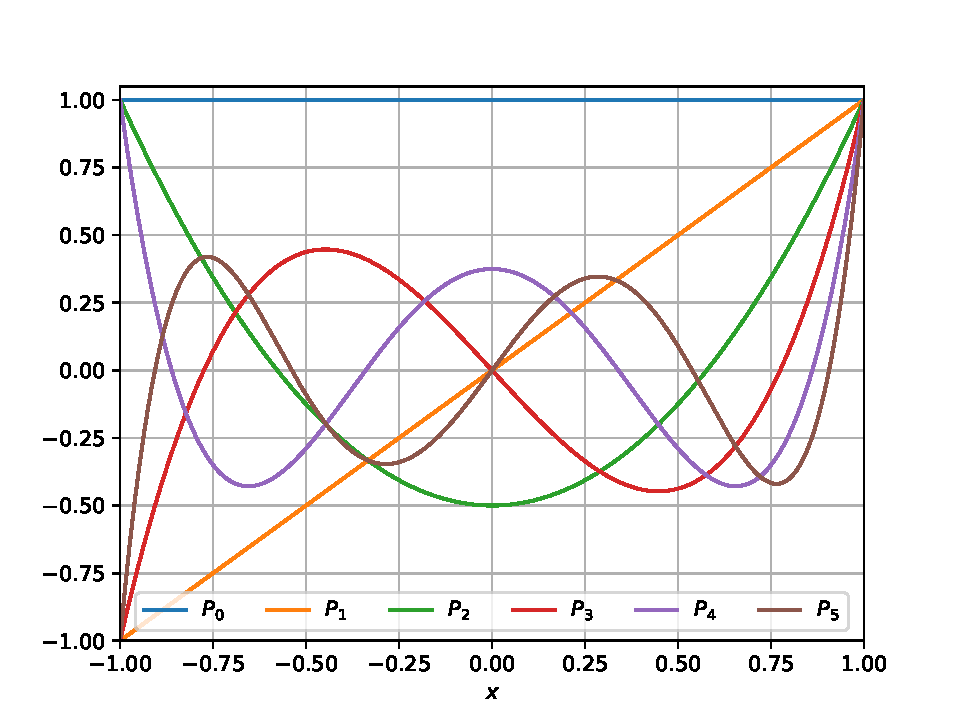
\includegraphics[width=0.75\columnwidth]{Figures/Legendre/Legendre_Plot.pdf}
		\caption{Plot of the first five Legendre polynomials.}
	\end{figure}

	\section{Associated Legendre Polynomials}
	The associated Legendre equation is
	\begin{equation}
		(1 - x^2)\dv[2]{y}{x} - 2x\dv{y}{x} + \left[l(l + 1) - \dfrac{m^2}{1 - x^2}\right]y = 0
	\end{equation}
	which can also be written as
	\begin{equation}
		\dv{x}\left[(1 - x^2)\dv{y}{x}\right] + \left[l(l + 1) - \dfrac{m^2}{1 - x^2}\right]y = 0
	\end{equation}
	The solutions to this differential equation is the associated Legendre polynomials, $ P_l^m(x) : [-1,1] \to \mathbb{R} $.\footnote{Similar to the unassociated Legendre polynomials, there is a second family of solutions known as the associated Legendre polynomials of the second kind. Again, they are not necessary to know within the scope of the compendium. Hence, they have also been neglected.} Similarly, they form an orthonormal basis. We have that
	\begin{equation}
		\int_{-1}^{1}P_l^m(x)P_{l'}^m(x)\dd{x} = \dfrac{2}{2l + 1}\dfrac{(l + m)!}{(l - m)!}\delta_{ll'}
	\end{equation}
	and
	\begin{equation}
		\int_{-1}^{1}P_l^m(x)P_l^{m'}(x)\dfrac{\dd{x}}{1 - x^2} = \dfrac{(l + m)!}{m(l - m)!}\delta_{mm'}
	\end{equation}
	For positive $ m $, we can define the associated Legendre polynomials using the unassociated Legendre polynomials given by
	\begin{equation}
		P_l^m(x) = (-1)^m(1 - x^2)^{m/2}\dv[m]{x}P_l(x)
	\end{equation}
	For negative $ m $,
	\begin{equation}
		P_l^{-m}(x) = (-1)^m\dfrac{(l - m)!}{(l + m)!}P_l^m(x)
	\end{equation}
	
	\section{Spherical Harmonics}
	\section{Bessel Functions of the First Kind}
	\section{Bessel Functions of the Second Kind}
	

\end{document}